\chapter{Architecture Overview For Cloud Computing With NETINF}
In Figure 1.1 it is shown how the basic cloud computing
service IaaS is composed of a set of virtualized resources,
namely CPU, memory, storage and network transport. In the
previous section, it is already explained how NetInf can
offer an enhanced solution for network transport and storage.
But let’s take one step back and look at the two main reasons
to virtualize resources: one is security - to restrict access to
resources in order to offer a ‘virtual private’ environment,
the other is resource separation in order to avoid resource
conflicts.

NetInf can offer an alternative to the security aspect of
virtualization for two of the cloud computing resources,
storage and network transport. The NetInf networking
architecture inherently secures the access to information
objects and network resources by cryptographic means.
There is therefore no need to virtualize storage and network
transport resources to ensure the access rights. This stems
from the fact that NetInf abstracts away the boxes and links
that are implementing these resources and secures the
resources themselves. Thus, there is no need to virtualize
these boxes and links from a security perspective.

The need to virtualize for resource separation may or
may not be a problem depending on the network
configuration. With the current trend of reduced prices,
especially on storage but also on transmission links, this
might be dealt with by traditional overprovisioning, which
can be combined with active network management in order
to ensure that new (real) resources are added before resource
conflicts appear. NetInf in combination with advanced
virtualization techniques like Vnet proposed in 4WARD can
provide a simpler solution to this problem by virtualizing
both storage and network transport resources. One key
advantage with Vnet compared to other virtualization
techniques is that it also addresses the problem of
virtualizing wireless network resources.

The NetInf architecture provides an API for
communication between arbitrary types of information
objects, independently of which hosts they are attached to,
and of how they move between hosts. Arbitrary
information object  means any information object which
adheres to the NetInf naming scheme, and which is
registered with the NetInf name resolution system. Examples
of such objects are data files, service objects, or digital
representations of physical objects, such as RFID tags.

The NetInf API supports a mode of communication
which is object-centric in the sense that only the object
identity or a set of attributes are needed to access an object.
The object naming scheme allows users and applications to
create object names based on cryptographic hashes of the
owner’s public key. This avoids the need for introducing a
new naming authority. Such object names are entirely
independent of the location of the object. Using this naming
scheme, the API hides the location of an object, as well as
the dynamics of the underlying transport network. In
addition, if several identical copies of an object exist in the
network, the NetInf name resolution and routing system
finds the "best" copy in an anycast fashion.

\begin{figure}[h]
\begin{center}
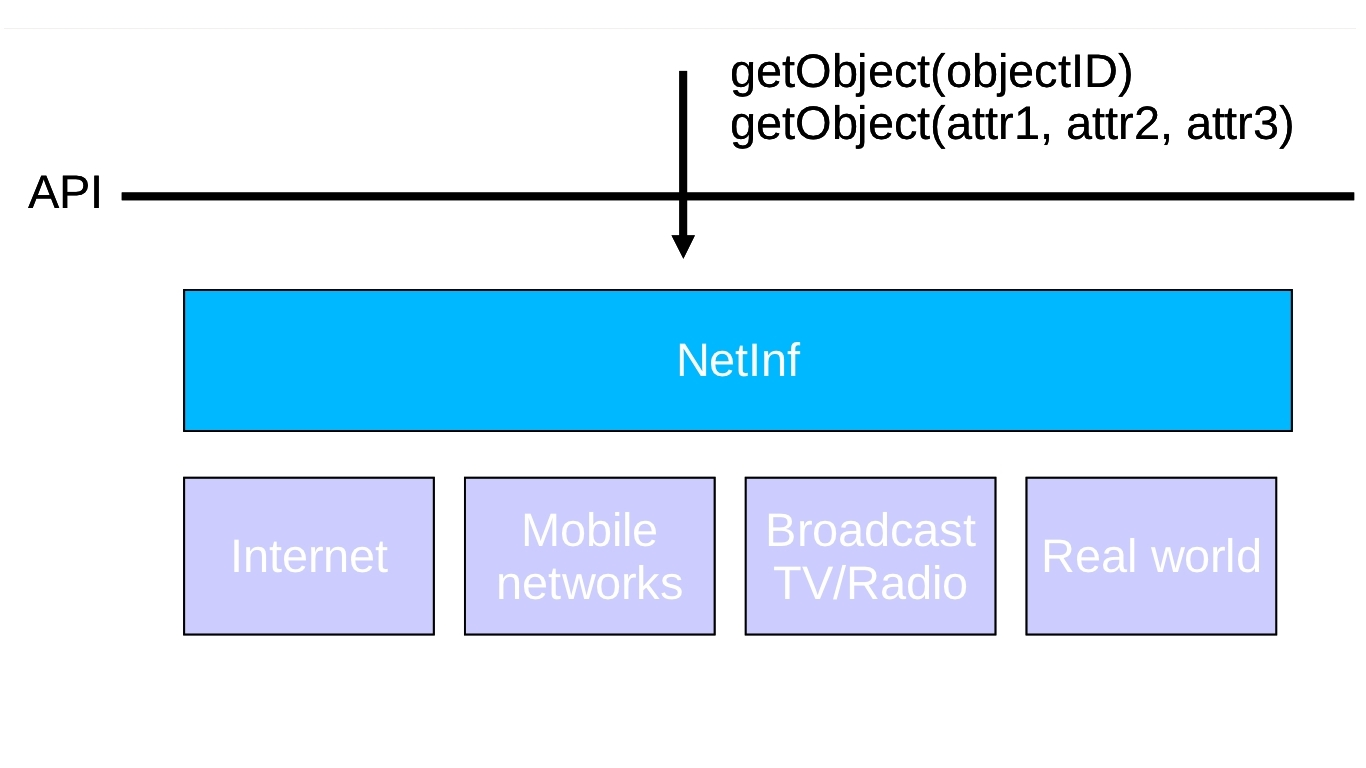
\includegraphics[height=6cm]{3.jpg}
\caption{NETINF API}
\end{center}
\end{figure}

The API includes methods such as publish(objectName),
resolve(objectName), and get(ObjectName). These methods
allow for registrations of objects in the name resolutions
system, resolving the location of an object, and establishing
connectivity with the object. The API also includes methods
for object storage and retrieval.

Figure 4.2 shows how NetInf can support a set of different
cloud computing services. The cloud computing service uses
NetInf objects, which communicate over a dynamic
infrastructure network, such as a global network, using the
NetInf API. The service uses object names to retrieve and
interact with other objects over the API, and has no notion of
object locators. The dynamic infrastructure network on the
other hand uses traditional addresses (locators), and has no
notion of service layer objects.


\begin{figure}[h]
\begin{center}
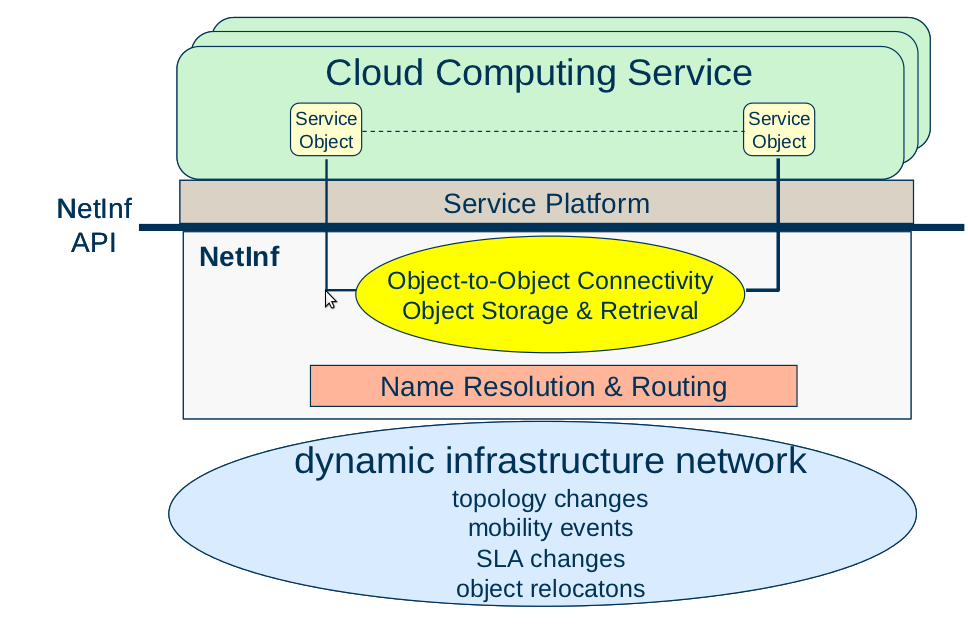
\includegraphics[height=8cm]{4.png}
\caption{Architecture Overview For The Support Of Cloud Computing}
\end{center}
\end{figure}

A cornerstone of the NetInf architecture is the name
resolution and routing system, which resolves the name of an
object to a set of current network locators. The resolution
mechanism is designed to handle highly dynamic network
topologies in a scalable fashion, and provides an updated
ocator for a digital object that is moved between hosts, or
for digital objects that are stored on mobile hosts, which in
turn may be attached to moving networks. Also, the
resolution mechanism is capable of handling multihoming of
objects, hosts, and networks. Note that the capability of
handling these rather general mobility and multihoming
scenarios also provides a basis for the handling of dynamic
events in fixed networks as described earlier.

The name resolution and routing system is designed to
scale to large networks and to a large number of objects. Likewise, the routing system must allow for short
convergence times also in a dynamic network topology. The
focus of the next section is on the name resolution and
routing system and its interoperation with the dynamic
network infrastructure. A novel mechanism is described that
allows for a strict separation between the object-centric view
of the API on the one hand, and a highly dynamic network
topology on the other hand.

